\epigraph{\textit{'A helicopter does not want to fly, it just vibrates so much that the ground rejects it.'}}{Kurt Vonnegut}

\section{Optimal control of pitch/travel and elevation with and without feedback (10.4)}

%%%%%%%%%%%%%%%%%%%%%%%%%%%%%%%%%%%%%%%%%%%%%%%%%%%%%%%%%%%%
\subsection{Discretisation with elevation states (10.4.1)} \label{10.4.1}
%%%%%%%%%%%%%%%%%%%%%%%%%%%%%%%%%%%%%%%%%%%%%%%%%%%%%%%%%%%%
We will re-formulate the continuous system \eqref{eq:system} with additional states for elevation ($e$) and elevation rate ($\dot{e}$). The system with new state and input vectors \eqref{eq:state_input} and state equations \eqref{eq:state_eqns} yield the matrices shown in \eqref{eq:matrices}.

\begin{equation}\label{eq:system}
	\V{\dot{x}}	= \M{A} \V{x} + \M{B} \V{u}
\end{equation}

\begin{equation}\label{eq:state_input}
	\V{x} =
	\begin{bmatrix}
		\lambda & r & p & \dot{p} & e & \dot{e}
	\end{bmatrix}\transpose
	,\qquad
	\V{u} =
	\begin{bmatrix}
		p_{c} & e_{c}
	\end{bmatrix}\transpose
\end{equation}

\begin{equation}\label{eq:state_eqns}
\begin{aligned}
	\dot{\lambda}	&= r \\
	\dot{r} 		&= - K_{2} p \\
	\dot{p}			&= \dot{p} \\
	\ddot{p}		&= K_{1} K_{pp} (p_{c} - p) - K_{1} K_{pd} \dot{p} \\
	\dot{e}			&= \dot{e} \\
	\ddot{e}		&= K_{3} K_{ep} (e_{c} - e) - K_{3} K_{ed} \dot{e}
\end{aligned}
\end{equation}

\begin{equation}\label{eq:matrices}
	\V{\dot{x}} =
	\underbrace{
		\begin{bmatrix}
			0 & 1 & 0				& 0				& 0				& 0				\\
			0 & 0 & -K_{2}			& 0				& 0				& 0				\\
			0 & 0 & 0				& 1				& 0				& 0				\\
			0 & 0 & -K_{1}K_{pp}	& -K_{1}K_{pd}	& 0				& 0				\\
			0 & 0 & 0				& 0 			& 0				& 1				\\
			0 & 0 & 0				& 0				& -K_{3}K_{ep}	& -K_{3}K_{ed}	\\
		\end{bmatrix}
	}_{\M{A}_{c}}
	\V{x} +
	\underbrace{
		\begin{bmatrix}
			0			& 0				\\
			0			& 0				\\
			0			& 0				\\
			K_{1}K_{pp}	& 0				\\
			0			& 0				\\
			0			& K_{3}K_{ep}	\\
		\end{bmatrix}
	}_{\M{B}_{c}}
	\V{u}
\end{equation}

%%%%%%%%%%%%%%%%%%%%%%%%%%%%%%%%%%%%%%%%%%%%%%%%%%%%%%%%%%%%
\subsection{Discretisation again (10.4.2)}
%%%%%%%%%%%%%%%%%%%%%%%%%%%%%%%%%%%%%%%%%%%%%%%%%%%%%%%%%%%%
As in section \ref{sec:disc1}, we again need to discretize the system. The result can be seen in \eqref{eq:matrix_4.2_A} and \eqref{eq:matrix_4.2_B}.

\begin{equation}
\begin{aligned}
	\V{x}_{k+1}	&= \V{x}_{k} + \left( \M{A}_{c} \V{x}_{k} + \M{B}_{c} \V{u}_{k} \right) h \\
				&= \underbrace{\left( \Mc{I} + h \M{A}_{c} \right)}_{\M{A}} \V{x}_{k}
				+ \underbrace{h \M{B}_{c}}_{\M{B}} \V{u}_{k} \\
\end{aligned}
\end{equation}

\begin{equation}\label{eq:matrix_4.2_A}
	\M{A} =
	\begin{bmatrix}
		1 & h & 0				& 0					& 0				& 0					\\
		0 & 1 & -hK_{2}			& 0					& 0				& 0					\\
		0 & 0 & 1				& h					& 0				& 0					\\
		0 & 0 & -hK_{1}K_{pp}	& 1-hK_{1}K_{pd}	& 0				& 0					\\
		0 & 0 & 0				& 0					& 1				& h					\\
		0 & 0 & 0				& 0					& -hK_{3}K_{ep}	& 1-hK_{3}K_{ed}	\\
	\end{bmatrix}
\end{equation}

\begin{equation}\label{eq:matrice_4.2_B}
	\M{B} =
	\begin{bmatrix}
		0				& 0				\\
		0				& 0				\\
		0				& 0				\\
		hK_{1}K_{pp}	& 0				\\
		0				& 0				\\
		0				& hK_{3}K_{ep}	\\
	\end{bmatrix}
\end{equation}

%%%%%%%%%%%%%%%%%%%%%%%%%%%%%%%%%%%%%%%%%%%%%%%%%%%%%%%%%%%%
\subsection{(10.4.3)}
%%%%%%%%%%%%%%%%%%%%%%%%%%%%%%%%%%%%%%%%%%%%%%%%%%%%%%%%%%%%

The cost function now has to include the elevation state, which gives us \eqref{eq:cost_function_w_elev}, with constrains given by \eqref{eq:cost_constraint_w_elev}. 

\begin{equation} \label {eq:cost_function_w_elev}
	\phi = \sum\limits_{i=1}^N (\lambda_i - \lambda_f)^2 + q_1 p_{ci}^2 + q2 e_{ci}^2
\end{equation}

\begin{equation} \label{eq:cost_constraint_w_elev}
	\alpha \exp (-\beta (\lambda_k - \lambda_t)^2) -e_k \leq 0, \quad k \in \{ 1, ..., N \}
\end{equation}

In \eqref{eq:cost_constraint_w_elev}, we used the values $\alpha = 0.2$, $\beta = 20$ and $\lambda_t = \frac{2 \pi}{3}$.
We use \texttt{fmincon} to get the result of the cost function with the constraints. The parameters we send it are  \texttt{vlb} and \texttt{vub}, which are vectors containing the linear constraints, \texttt{mycon}, which returns the nonlinear constraints and \texttt{Aeq} and \texttt{beq} which are the matrices for the problem to be solved. We also send in the cost function itself and the start values \texttt{z0}.
\begin{lstlisting}
costf = @(z) 0.5*z'*Q*z;
z = fmincon(costf, z0, [], [], Aeq, beq, vlb, vub, @mycon);
\end{lstlisting}

%%%%%%%%%%%%%%%%%%%%%%%%%%%%%%%%%%%%%%%%%%%%%%%%%%%%%%%%%%%%
\subsection{Comparison of performance with and without feedback(10.4.4)}
%%%%%%%%%%%%%%%%%%%%%%%%%%%%%%%%%%%%%%%%%%%%%%%%%%%%%%%%%%%%
Without feedback the pitch goes to 0 when $\lambda = \lambda_f$, but does not compensate to stop the helicopter from traveling past $\lambda = \lambda_f$. With feedback, the helicopter will change its pitch to the opposite direction, thus making the helicopter stop and stay still at $\lambda = \lambda_f$. 

\begin{figure}[H]
	\centering
	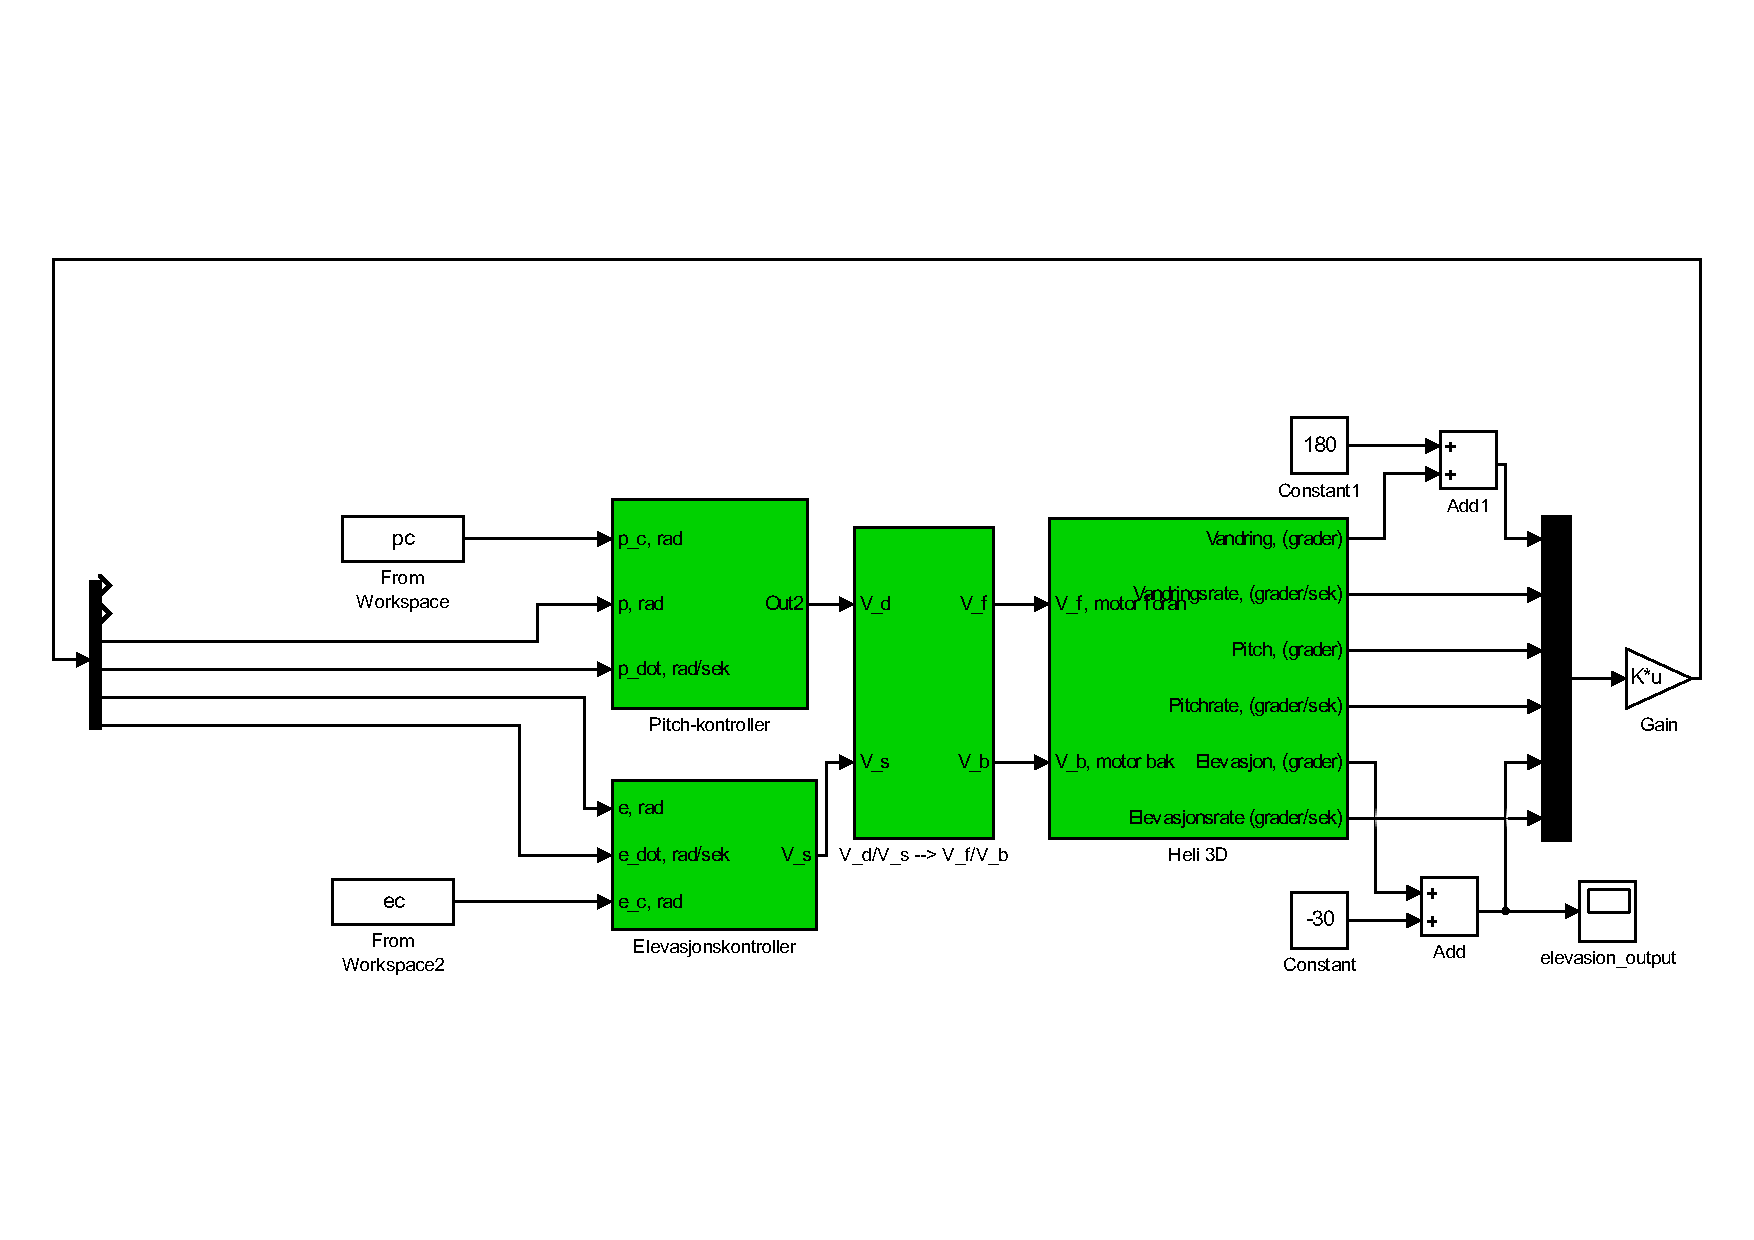
\includegraphics[width=\textwidth, trim=2cm 5cm 2cm 2cm]{simulinkmodels/heldag4UnFeed}
	\caption{Simulink model of the system without feedback}
	\label{fig:heldag4UnFeed}
\end{figure}

\begin{figure}[H]
	\centering
	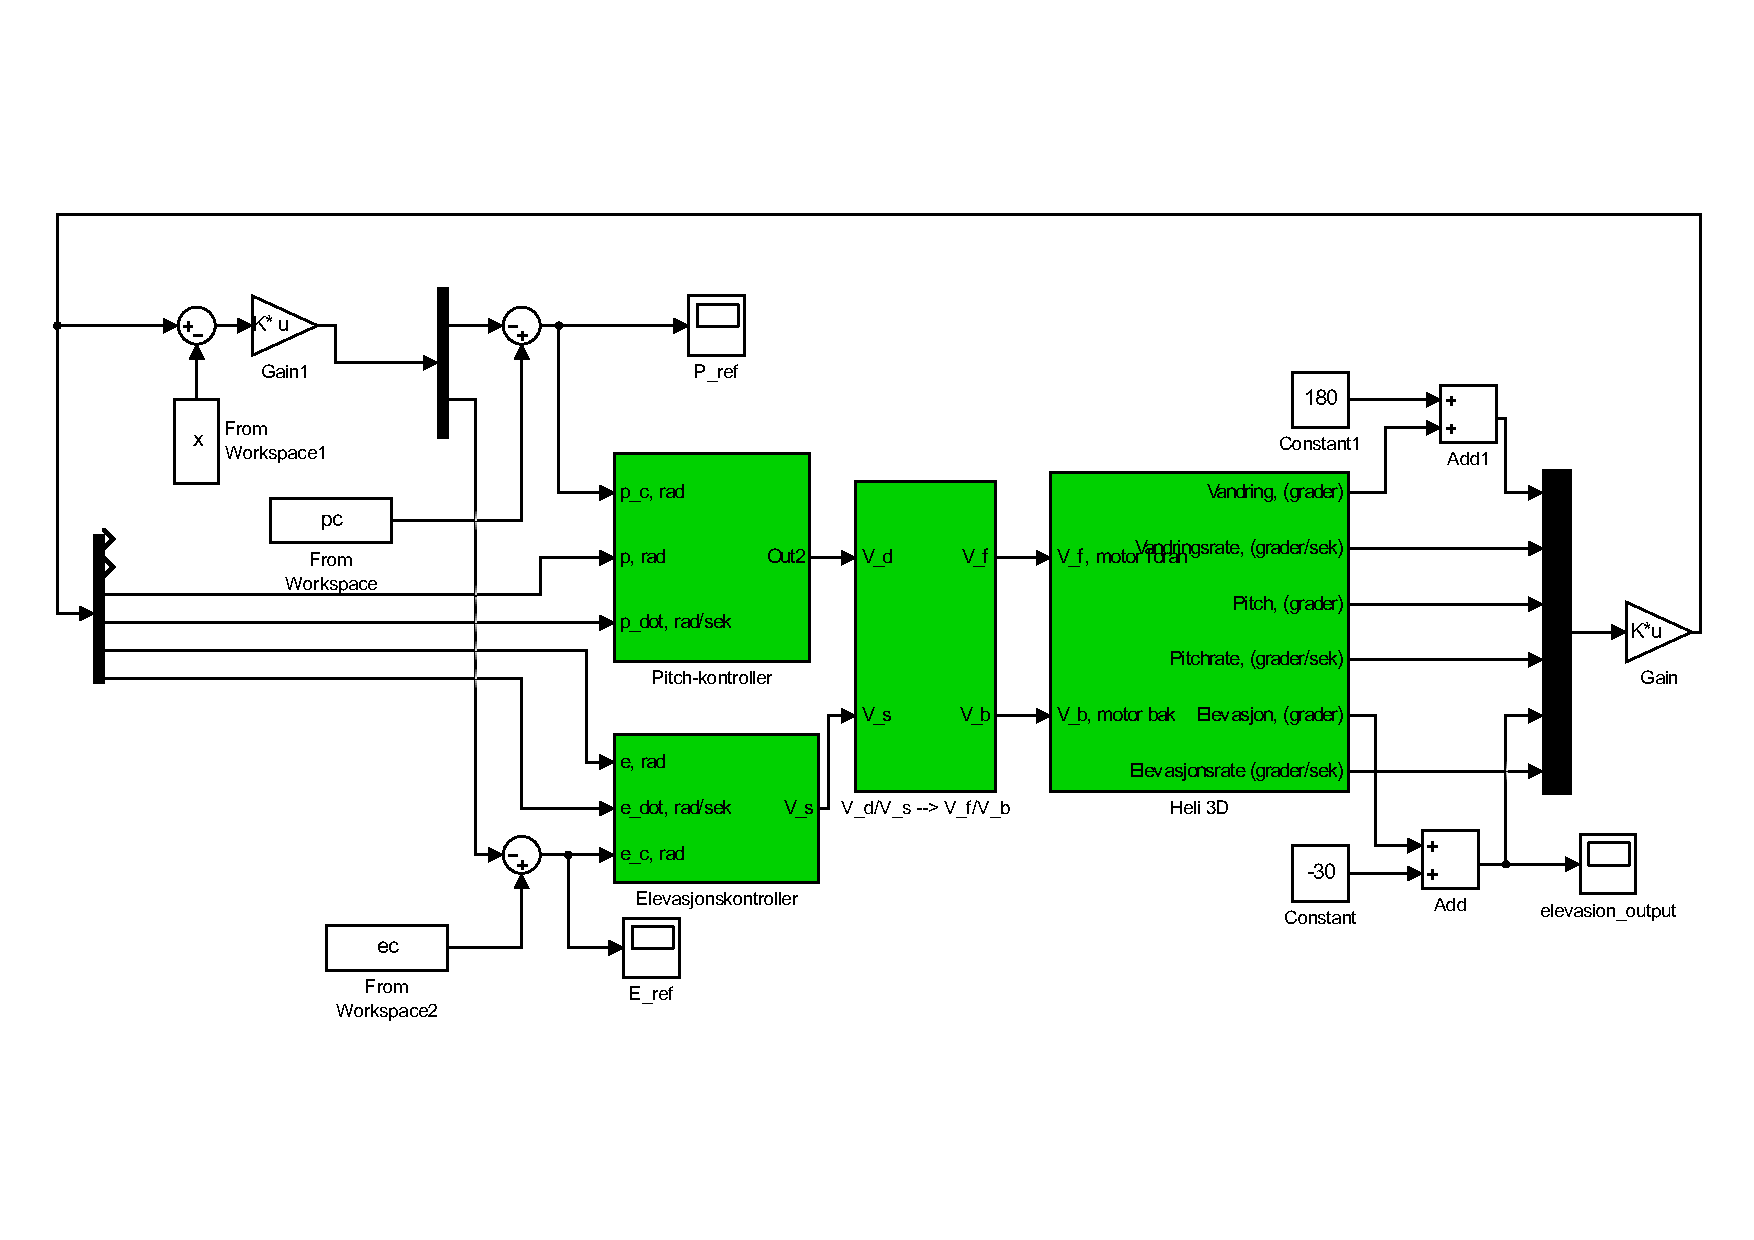
\includegraphics[width=\textwidth, trim=2cm 5cm 2cm 2cm]{simulinkmodels/heldag4medFeed}
	\caption{Simulink model of the system with feedback}
	\label{fig:heldag4medFeed}
\end{figure}
TODO add plots to compare


\begin{figure}[H]
	\centering
	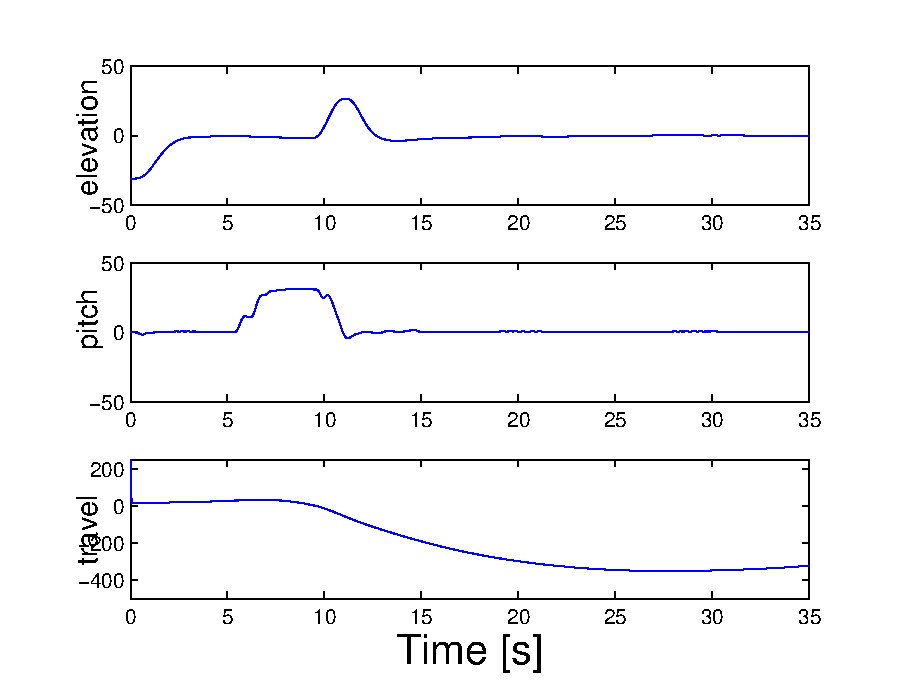
\includegraphics[width=\textwidth]{day4_nofeed}
	\caption{Actual values day 4 without feedback}
	\label{fig:day4nofeed}
\end{figure}


\begin{figure}[H]
	\centering
	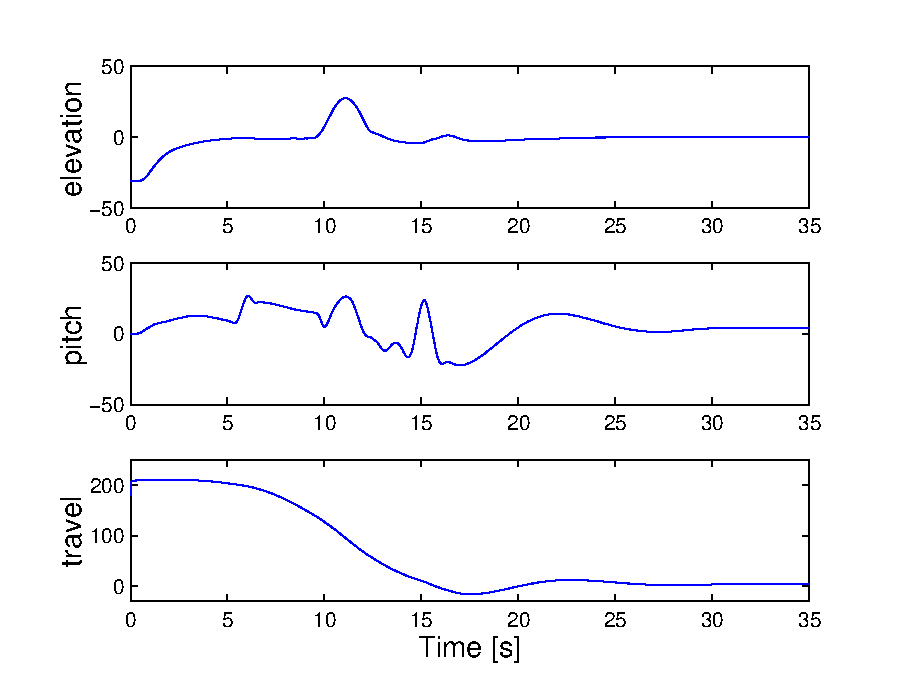
\includegraphics[width=\textwidth]{day4_yesfeed}
	\caption{Actual values day 4 with feedback}
	\label{fig:day4yesfeed}
\end{figure}

%%%%%%%%%%%%%%%%%%%%%%%%%%%%%%%%%%%%%%%%%%%%%%%%%%%%%%%%%%%%
\subsection{(10.4.5)}
%%%%%%%%%%%%%%%%%%%%%%%%%%%%%%%%%%%%%%%%%%%%%%%%%%%%%%%%%%%%
In real life the pitch and pitch rate of the helicopter would have an effect on both the elevation rate and elevation itself. This will make the helicopter get an offset on where it goes compared to the calculated optimal trajectory.  
By modeling the system with the elevation and travel coupled with the pitch, you will remove the offset at the cost of a more complex model.